\documentclass[12pt,a4paper,brazilian, fleqn]{article}

\usepackage{babel}
\usepackage[utf8]{inputenc}
\usepackage[T1]{fontenc}
\usepackage{lmodern}

\usepackage{amssymb,amsfonts,amsmath}

\usepackage{tikz}
\usetikzlibrary{calc,intersections}

%https://tex.stackexchange.com/a/100406
%29.7 cm - 1cm - 1cm - 144.90/28.4 cm = 22.60 cm
\usepackage[a4paper, totalheight=22.60cm,includeheadfoot,left=1.5cm, right=1.0cm, top=1cm]{geometry}
\setlength{\headheight}{144.90pt}

\setkeys{Gin}{keepaspectratio}

\newcommand{\cabeca}{
    \begin{tikzpicture}
        \node(Logo) {
\includegraphics[width=2.5cm]{logo.png}};
        % \node(Logo) {
\includegraphics[width=4.1cm]{logo.png}};

        \node(Local) at (Logo.north east) [anchor=north west, yshift=-0.25cm,
            align=center, execute at begin node=\setlength{\baselineskip}{3ex}]
            {
                \huge{\textbf{Universidade Federal do Amazonas}} \\
                \large{\textbf{Instituto de Ciências Exatas e Tecnologia}} \\
                \large{\textbf{\Description}}
            };

        \node(Ident) at (Local.south west) [anchor=north west, yshift=-0.25cm,
            align=left, execute at begin node=\setlength{\baselineskip}{2em}]
            {
                Professor: {\fontfamily{augie}\selectfont \Professor} \\
                Aluno(s):
            };
        % \draw [thick] (Logo.south west) -- ($(Logo.south west -| Local.south east)$);
        % \draw [red] (Logo.north west) rectangle (Logo.south east);
        % \draw [blue] (Local.north west) rectangle (Local.south east);
        % \draw [green] (Ident.north west) rectangle (Ident.south east);
    \end{tikzpicture}
}

\usepackage{fancyhdr}
\fancyhead{}
\fancyfoot{}
\fancyhead[c]{\cabeca}
\fancyfoot[r]{\fontfamily{augie}\selectfont Boa sorte!}

\pagestyle{fancy}
\renewcommand{\headrulewidth}{0pt}
\renewcommand{\footrulewidth}{0pt}

\newcommand{\ratio}[1]{(#1\% da nota)}
%-----------------------------------CUT HERE-----------------------------------

\def\Description{Física Geral II -- Prova Final}
\def\Professor{Rodrigo de Farias Gomes}

\usepackage{siunitx}
\sisetup{locale = FR}

\usepackage{tcolorbox}
\tcbset{boxrule=0pt, top=0pt, bottom=0pt}

\DeclareMathOperator{\sen}{sen}
\DeclareMathOperator{\tg}{tg}
\usepackage{enumitem}
\usepackage{calc}

\begin{document}

\begin{tcolorbox}[colback=black!10, colframe=black!50, title=Observações]
    \begin{itemize}
        \item Todas as páginas com resposta devem ter o nome e matrícula do
            aluno escritos com caneta no início (cabeçalho) ou no final
            (rodapé). Páginas que não obedeçam a esse critério não serão usadas
            na avaliação
    \end{itemize}
\end{tcolorbox}

\vspace{2em}

\begin{enumerate}

        \begin{minipage}{0.45\textwidth}
        \item \ratio{33} Na figura ao lado, uma amostra de gás se expande de \(V_0\) para
            \(4V_0\) enquanto a pressão diminui de \(p_0\) para \(p_0/4\). Se \(V_0 = \SI{1.25}{m^3}\)
            e \(p_0=\SI{60}{Pa}\), qual é o trabalho realizado pelo gás se a pressão varia 
            com o volume de acordo (a) com a trajetória \(A\), (b) com a trajetória \(B\) e
            (c) com a trajetória \(C\)?
        \end{minipage}%
        \begin{minipage}{0.45\textwidth}
            \centering
            \begin{tikzpicture}
                \node [inner sep=0] (A) {
                    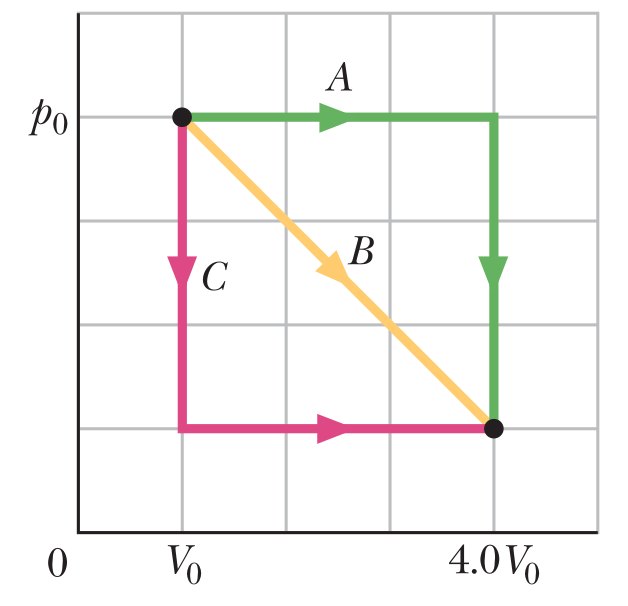
\includegraphics[width=0.75\textwidth]{Captura de tela de 2025-07-08 16-01-05.png}
                };
                \path (A.south west) -- (A.north west) node [midway, sloped] {Pressão (\si{Pa})};
                \path (A.south west) -- (A.south east) node [midway, yshift=-1ex] {Volume (\(\si{m^3}\))};
            \end{tikzpicture}
        \end{minipage}

    \item \ratio{33} Um bloco de cobre, de \(\SI{50}{g}\), cuja a temperatura é 
        \SI{117}{\celsius}, é colocado em uma caixa isolada junto com um bloco de chumbo de 
        \SI{100}{g} cuja temperatura é \SI{-80}{\celsius}. (a) Qual é a temperatura de equilíbrio
        do sistema de dois blocos? (b) Qual é a variação da energia interna do sistema 
        do estado inicial para o estado de equilíbrio? (c) Qual é a variação da 
        entropia do sistema?

    \item \ratio{34} Uma mistura de \SI{1773}{g} de água e \SI{327}{g} de gelo
        está inicialmente em equilíbrio a \SI{0}{\celsius}. A mistura é levada,
        por um processo reversível, a um segundo estado de equilíbrio no qual a 
        razão água-gelo, em massa, é 2:1 a \SI{0}{\celsius}. (a) Calcule a variação 
        de entropia do sistema durante esse processo. (b) O sistema é levado de volta
        ao estado de equilíbrio inicial por um processo irreversível (usando, por
        exemplo, um bico de Bunsen). Calcule a variação de entropia do sistema durante
        esse processo. (c) As respostas dos itens (a) e (b) são compatíveis com a 
        segunda lei da termodinâmica?

\end{enumerate}

Dados:
\begin{itemize}
    \item Calor específico do chumbo: \(\SI{128}{J/kg\cdot K}\)
    \item Calor específico do cobre: \(\SI{386}{J/kg\cdot K}\)
    \item Calor de fusão da água: \(\SI{333}{kJ/kg}\)
\end{itemize}
\end{document}
